\chapter{Music Theory}

\section{Structure}

\subsection{Scale}
A scale is division of a octave into a collection of notes. The two primary classes of scales are major and minor. 
\begin{enumerate}
    \item Major: W,W,H,W,W,W,H
    \item Minor: W,H,W,W,H,W,W
\end{enumerate}

\subsection{Key}
Key can be thought of as the root note or tonic of a scale. To shift between keys a commonality is needed for a smooth transition whether it be note or chord. For instance C major to G major; see Figure \ref{fig:fifths} as reference between key transitions.

\begin{figure}[htbp]
    \centering
    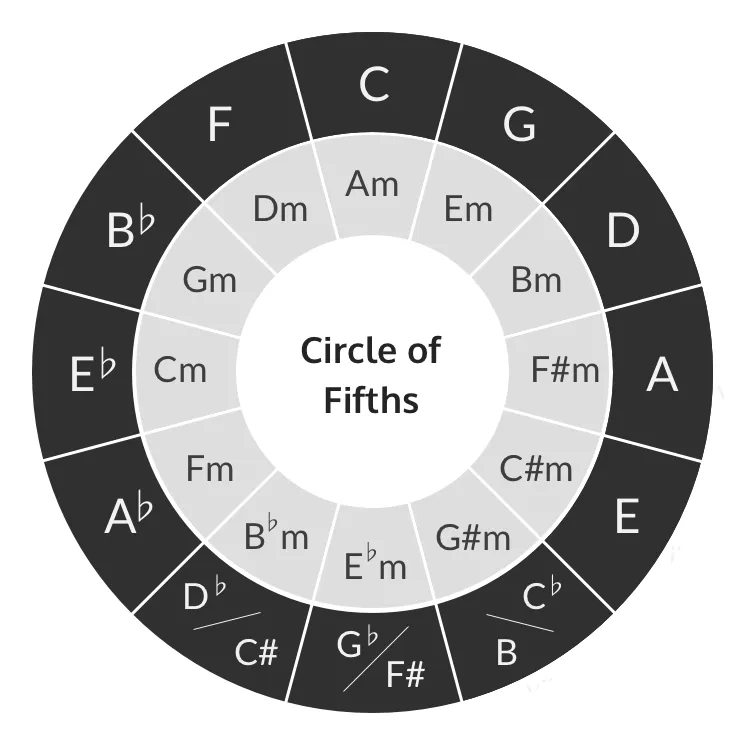
\includegraphics[width=0.8\textwidth]{Images/circle-of-fifths-full.png}
    \caption{Circle of fifths}
    \label{fig:fifths}
\end{figure}